\subsection{Data}


\begin{frame}{Property Matching}
    \begin{figure}
        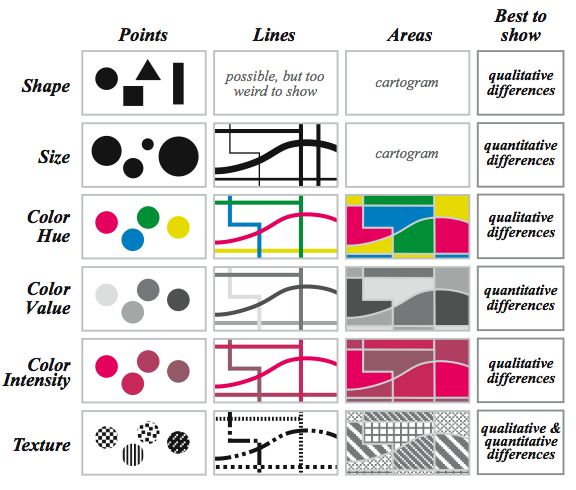
\includegraphics[width=.7\textwidth]{figures/intro/retinal_variables.png}
        \caption{This tabular form of Bertin's retinal variables is from Understanding Graphics \cite{malamedInformationDisplayTips2010} who reproduced it from Krygier and Wood's \textit{Making Maps: A Visual Guide to Map Design for GIS}\cite{krygierMakingMapsVisual2005}}
    \end{figure}
\end{frame}

\begin{frame}{Visualization is commutative maps}

    \pause
    %% deconstruct D\R\V
    \begin{center}
        \textbf{Tam: Add topology and make it functional}
    \end{center}
\end{frame}
\begin{frame}{Evaluating visualizations}
    \begin{description}
        \item[Expressiveness] structure preserving mappings from data to graphic (Mackinlay \cite{mackinlayAutomatingDesignGraphical1986})
        \item[Effectiveness] design choices made in deference to perceptual saliency \cite (Mackinlay \cite{clevelandResearchStatisticalGraphics1987,clevelandGraphicalPerceptionTheory1984,chambersGraphicalMethodsData1983a, munznerVisualizationAnalysisDesign2014})
        \item[Naturalness] easier to understand when properties match (Norman \cite{norman_things_smart})
        \item[Graphical Integrity] graphs show \textbf{only} the data (Tufte \cite{tufteVisualDisplayQuantitative2001})
    \end{description}
\end{frame}

\begin{frame}{Mathematical Frameworks for evaluating visualization}
    \begin{enumerate}
        \item APT: visualization has syntax and semantics like a language  (Mackinlay  \cite{mackinlayAutomatingDesignGraphical1986, mackinlayAUTOMATICDESIGNGRAPHICAL1987})
        \item visualization has functional dependencies that can be represented as graphs (Sugibuchi \cite{sugibuchiFramwork2009}) 
        \item the semiotics of visualization are commutative in a category theory framework (Vickers \cite{vickersUnderstandingViz2013})
        \item data ($\alpha$) and viz ($\omega$) symmetries (Kindlmann and Scheidegger \cite{kindlmann2014algebraic})
        \begin{block}{$v\circ r_2 \circ \alpha =\omega\circ v\circ r_1$}
            \begin{equation*}
            \begin{tikzcd}[ampersand replacement=\&]
                D \arrow[d, "\alpha"'] \arrow[r, "r_1"] \& R \arrow[r, "\nu"]  \& V \arrow[d, "\omega"] \\
                D \arrow[r, "r_2"']                     \& R \arrow[r, "\nu"'] \& V                    
            \end{tikzcd}
            \end{equation*}
        \end{block}
\end{frame}
